% Provenance (never printed): see sources/outline_sources.md (Year 1:
% astronomy of position, spherical trigonometry, time scales, insolation).
% Spherical trigonometry is absent from the mathematics series: this chapter
% owns it. Curves computed in figdata/bachelor-1/{sun_paths, day_length,
% celestial_sphere, spherical_triangle}.py (shared model _solar.py); numbers
% of the exercises and problem in the Book 3 scratch calculator ch01.py.
\chapter{Sferische astronomie}\label{ch:b1:spherical-astronomy}

Op een heldere nacht ver van elke stad registreert een camera met een lange
belichtingstijd, op de hemel gericht, de sterren als bogen van cirkels die
allemaal om één punt staan dat niet beweegt. Een ster die vanavond om negen
uur in het oosten opkwam, komt morgen om ongeveer vijf voor negen op, en elke
nacht daarna iets eerder. De zon staat om twaalf uur 's middags in juni hoger
dan in december, en in het verre noorden gaat zij midden in de zomer helemaal
niet onder. Dit alles is de draaiing van de aarde en haar baan om de zon, vanaf
de grond gezien. Om het te beschrijven hebben de astronoom en de
geowetenschapper coördinaten op een bol nodig, de trigonometrie van driehoeken
op een bol en klokken die gelijke tred houden met de sterren of met de zon.
Dit hoofdstuk bouwt die hulpmiddelen. Ze keren terug in de plaatkinematica
(\cref{ch:b1:plate-kinematics}), waar platen over de bol draaien, en in de
klimaathoofdstukken (\cref{ch:b1:radiation-heat-transport}), waar het zonlicht
dat een \omterm{def:b1:spherical-astronomy:geographic}{breedtegraad} ontvangt de winden en de stromingen aandrijft.

\begin{recall}
De aarde draait eenmaal per dag om haar as en beweegt in een jaar om de zon,
op een baan die vrijwel een cirkel is. Haar as staat schuin ten opzichte van
de baan, en dat veroorzaakt de seizoenen (de natuurkundeboeken, klassen 6 en 12;
de wetten van Kepler komen aan bod in het eerste jaar van de natuurkundeboeken
voor het hoger onderwijs). Een punt op aarde wordt bepaald door zijn
\omterm{def:b1:spherical-astronomy:geographic}{breedtegraad} en \omterm{def:b1:spherical-astronomy:geographic}{lengtegraad} (Boek 1, klas 6). Een vector met lengte één wordt
vastgelegd door twee hoeken, zoals in bolcoördinaten; het inproduct van twee
eenheidsvectoren is de cosinus van de hoek ertussen, en het drievoudig product
$\vec u\cdot(\vec v\times\vec w)$ blijft gelijk bij een cyclische verwisseling
van de drie vectoren.
\end{recall}

\section{Driehoeken op een bol}

\begin{definition}[Grootcirkel, sferische driehoek]\label{def:b1:spherical-astronomy:spherical-triangle}
Een \emph{grootcirkel}\index{grootcirkel} van een bol is de doorsnede met een
vlak door het middelpunt; elke andere vlakdoorsnede is een
\emph{kleine cirkel}\index{kleine cirkel}. Door twee punten die niet
tegenover elkaar liggen gaat precies één grootcirkel, en de kortste van de
twee bogen daarvan is de kortste weg over de bol tussen de punten. Een
\emph{sferische driehoek}\index{sferische driehoek} is de figuur die gevormd
wordt door drie punten van de bol, de hoekpunten $A$, $B$, $C$, verbonden door
bogen van grootcirkels die kleiner zijn dan \ang{180}. Zijn zijden $a$, $b$, $c$
(tegenover $A$, $B$, $C$) worden gemeten door de hoeken die zij opspannen in
het middelpunt; zijn hoeken $A$, $B$, $C$ zijn de hoeken tussen de vlakken van
de zijden die in elk hoekpunt samenkomen.
\end{definition}

Op de bol met straal $R$ heeft een zijde van $a$ radialen de lengte $Ra$. Elke
zijde en elke hoek ligt tussen $0$ en $\pi$.

\begin{omfigure}
\begin{tikzpicture}
\begin{axis}[x=1cm, y=1cm, hide axis, xmin=-2.7, xmax=2.7, ymin=-2.6, ymax=2.6, clip=false]
\draw[black, line width=0.6pt] (axis cs:0,0) circle (2.4cm);
\addplot[black!45, densely dashed, line width=0.4pt] coordinates {(0,0) (-0.078358,1.7847)};
\addplot[black!45, densely dashed, line width=0.4pt] coordinates {(0,0) (-1.5903,-0.2902)};
\addplot[black!45, densely dashed, line width=0.4pt] coordinates {(0,0) (1.4453,-0.16381)};
\addplot[omDef, line width=1.1pt] table {figdata/out/bachelor-1-spherical_triangle-ab.dat};
\addplot[omDef, line width=1.1pt] table {figdata/out/bachelor-1-spherical_triangle-bc.dat};
\addplot[omDef, line width=1.1pt] table {figdata/out/bachelor-1-spherical_triangle-ca.dat};
\addplot[omThm, line width=0.8pt] table {figdata/out/bachelor-1-spherical_triangle-angA.dat};
\addplot[only marks, mark=*, mark size=1.4pt] table[x=x, y=y] {figdata/out/bachelor-1-spherical_triangle-verts.dat};
\fill (axis cs:0,0) circle (1.2pt);
\begin{scope}[font=\small]
  \node[above] at (axis cs:-0.078358,1.7847) {$A$};
  \node[left] at (axis cs:-1.5903,-0.2902) {$B$};
  \node[right] at (axis cs:1.4453,-0.16381) {$C$};
  \node[above left] at (axis cs:0,0) {$O$};
  \node[omThm] at (axis cs:0.24,1.36) {$A$};
  \node[omDef] at (axis cs:0.0,-0.52) {$a$};
  \node[omDef] at (axis cs:0.95,0.95) {$b$};
  \node[omDef] at (axis cs:-1.05,0.95) {$c$};
\end{scope}
\end{axis}
\end{tikzpicture}

{\small Een \omterm{def:b1:spherical-astronomy:spherical-triangle}{sferische driehoek} $ABC$ op een bol met middelpunt $O$. De zijden $a$,
$b$, $c$ zijn bogen van \omterm{def:b1:spherical-astronomy:spherical-triangle}{grootcirkels}, gemeten door de hoeken $BOC$, $COA$,
$AOB$; de hoek $A$ (rood) is de hoek tussen de twee zijden die in
$A$ samenkomen. De getekende driehoek heeft $a = \ang{78.6}$, $b = \ang{62.6}$,
$c = \ang{64.8}$ en hoeken van \ang{89.9}, \ang{64.9} en \ang{67.4}, die samen
meer dan \ang{180} zijn.}
\end{omfigure}

\begin{theorem}[De cosinusregel]\label{thm:b1:spherical-astronomy:cosine-rule}
In een \omterm{def:b1:spherical-astronomy:spherical-triangle}{sferische driehoek} geldt
\[
  \cos a = \cos b\cos c + \sin b\sin c\cos A .
\]
\end{theorem}

\begin{proof}
Werk op de eenheidsbol en kies de assen zo dat $A$ in de pool ligt:
$\vec A = (0, 0, 1)$, en het vlak $xz$ dat $B$ bevat:
$\vec B = (\sin c, 0, \cos c)$, want $B$ ligt op hoekafstand $c$ van
$A$. Het punt $C$ ligt op hoekafstand $b$ van $A$, op een \omterm{def:b1:spherical-astronomy:spherical-triangle}{grootcirkel}
door $A$ die de hoek $A$ maakt met het vlak $xz$:
$\vec C = (\sin b\cos A, \sin b\sin A, \cos b)$. De zijde $a$ is de hoek tussen
$\vec B$ en $\vec C$, dus
\[
  \cos a = \vec B\cdot\vec C = \sin c\sin b\cos A + \cos c\cos b. \qedhere
\]
\end{proof}

\begin{theorem}[De sinusregel]\label{thm:b1:spherical-astronomy:sine-rule}
In een \omterm{def:b1:spherical-astronomy:spherical-triangle}{sferische driehoek} geldt
\[
  \frac{\sin A}{\sin a} = \frac{\sin B}{\sin b} = \frac{\sin C}{\sin c}.
\]
\end{theorem}

\begin{proof}
Met de vectoren van het vorige bewijs geldt
$\vec B \times \vec C = (-\cos c\sin b\sin A,\ \cos c\sin b\cos A - \sin c\cos b,\
\sin c\sin b\sin A)$, dus het drievoudig product is
$\vec A\cdot(\vec B\times\vec C) = \sin b\sin c\sin A$. Het drievoudig product
blijft gelijk bij een cyclische verwisseling van $A$, $B$, $C$. Door $B$ en
daarna $C$ in de pool te leggen volgt op dezelfde manier $\sin c\sin a\sin B$ en
$\sin a\sin b\sin
C$. De drie uitdrukkingen zijn gelijk; delen door
$\sin a\sin b\sin c$ geeft de regel.
\end{proof}

Als de zijden klein zijn ten opzichte van de straal, geldt $\cos a \approx 1 -
a^2/2$ en $\sin a \approx a$, en worden de twee regels de cosinus- en
sinusregel van vlakke driehoeken: op een voldoende klein stuk is de bol vlak.
Bij een grote driehoek gebeurt dat niet: de hoeken van een
\omterm{def:b1:spherical-astronomy:spherical-triangle}{sferische driehoek} tellen op tot meer dan \ang{180}
(\cref{exo:b1:spherical-astronomy:12}).

\begin{method}[Afstand en koers op de bol]\label{met:b1:spherical-astronomy:great-circle}
Om de kortste afstand te vinden tussen twee plaatsen met breedtegraden $\varphi_1$,
$\varphi_2$ en lengtegraden $\lambda_1$, $\lambda_2$, en de richting waarin men moet vertrekken:
\begin{enumerate}
  \item vorm de driehoek met als hoekpunten de Noordpool $P$ en de twee
        plaatsen; haar zijden vanaf de pool zijn de poolafstanden $\ang{90} -
        \varphi_1$ en $\ang{90} - \varphi_2$, en haar hoek bij de pool is het
        verschil in lengte $\Delta\lambda$;
  \item de cosinusregel geeft de hoekafstand $\Delta$:
        $\cos\Delta = \sin\varphi_1\sin\varphi_2 +
        \cos\varphi_1\cos\varphi_2\cos\Delta\lambda$; de afstand is
        $R\Delta$ ($\Delta$ in radialen);
  \item de beginkoers is de hoek van de driehoek bij de eerste plaats, uit
        de cosinusregel toegepast op de zijde er tegenover,
        $\sin\varphi_2 = \sin\varphi_1\cos\Delta + \cos\varphi_1\sin\Delta\cos
        \mathrm{Az}$, en wordt gemeten vanaf het noorden naar de tweede plaats.
\end{enumerate}
De koers verandert langs de \omterm{def:b1:spherical-astronomy:spherical-triangle}{grootcirkel} (behalve langs een meridiaan of de
evenaar): een schip of vliegtuig dat dezelfde kompaskoers aanhoudt, volgt een
andere, langere kromme.
\end{method}

\section{Coördinaten op de bol}

\begin{definition}[Breedtegraad en lengtegraad]\label{def:b1:spherical-astronomy:geographic}
Stel dat de aarde een bol is die om haar poolas draait. De
\emph{breedtegraad}\index{breedtegraad} $\varphi$ van een punt is de hoek tussen
het evenaarsvlak en de straal door het punt, van \ang{-90}
(Zuidpool) tot \ang{+90} (Noordpool); de \emph{lengtegraad}\index{lengtegraad}
$\lambda$ is de hoek, gemeten in het evenaarsvlak, tussen het meridiaanvlak van
het punt en dat van een referentiemeridiaan, die door Greenwich gaat, positief
naar het oosten, van \ang{-180} tot \ang{180}.
\end{definition}

De aarde is in feite iets afgeplat; de \omterm{def:b1:spherical-astronomy:geographic}{breedtegraad} die voor kaarten en voor de
hemel gebruikt wordt, is de hoek tussen de plaatselijke verticaal en het
evenaarsvlak. Die wijkt van de geocentrische hoek af met hoogstens \ang{0.2}
(\cref{ch:b1:isostasy-gravity}). Lijnen van gelijke breedte, de parallellen,
zijn \omterm{def:b1:spherical-astronomy:spherical-triangle}{kleine cirkels}; de meridianen zijn halve \omterm{def:b1:spherical-astronomy:spherical-triangle}{grootcirkels}.

\begin{definition}[De hemelbol]\label{def:b1:spherical-astronomy:celestial-sphere}
De \emph{hemelbol}\index{hemelbol} is een denkbeeldige bol met het middelpunt
in de waarnemer, waarop elke ster in haar richting ligt; alleen richtingen
tellen, niet afstanden. De verlengingen van de aardas snijden de bol in de
noordelijke en zuidelijke \emph{hemelpolen}\index{hemelpool}; het vlak van de
aardevenaar snijdt de bol langs de \emph{hemelevenaar}\index{hemelevenaar}. Het
\emph{zenit}\index{zenit} is het punt recht boven de waarnemer, langs de
plaatselijke verticaal; de horizon is de \omterm{def:b1:spherical-astronomy:spherical-triangle}{grootcirkel} op $\ang{90}$ ervan
vandaan. De \emph{plaatselijke meridiaan}\index{plaatselijke meridiaan} is de
\omterm{def:b1:spherical-astronomy:spherical-triangle}{grootcirkel} door het zenit en de hemelpolen; hij snijdt de horizon in het
noorden en het zuiden.
\end{definition}

Terwijl de aarde van west naar oost draait, lijkt de \omterm{def:b1:spherical-astronomy:celestial-sphere}{hemelbol} de andere kant op
te draaien, van oost naar west, om de as van de \omterm{def:b1:spherical-astronomy:celestial-sphere}{hemelpolen}, in iets minder dan
een dag. De sterren behouden hun onderlinge plaatsen: ze staan zo ver weg dat
een reis van een jaar om de zon hun richtingen minder dan een boogseconde
verandert (\cref{ch:b1:observing-the-sky}).

\begin{definition}[Horizontale coördinaten]\label{def:b1:spherical-astronomy:horizontal}
De \emph{hoogte}\index{hoogte (van een ster)} $h$ van een ster is haar hoek boven
de horizon, van \ang{-90} tot \ang{90}; haar zenithoek is
$z = \ang{90} - h$. Haar \emph{azimut}\index{azimut} $\mathrm{A}$ is de hoek,
langs de horizon, van het noorden tot de voet van de verticaalcirkel van de
ster, gemeten van \ang{0} tot \ang{360} via het oosten.
\end{definition}

Horizontale coördinaten zijn die van de waarnemer: ze veranderen met de plaats
en het tijdstip. De coördinaten van de hemel zelf worden meegevoerd door haar
draaiing.

\begin{definition}[Equatoriale coördinaten]\label{def:b1:spherical-astronomy:equatorial}
De \emph{declinatie}\index{declinatie (hemel)} $\delta$ van een ster is haar
hoek ten opzichte van de \omterm{def:b1:spherical-astronomy:celestial-sphere}{hemelevenaar}, positief naar het noorden, van \ang{-90}
tot \ang{90}. De \omterm{def:b1:spherical-astronomy:spherical-triangle}{grootcirkel} door de ster en de \omterm{def:b1:spherical-astronomy:celestial-sphere}{hemelpolen} is haar
uurcirkel. De \emph{uurhoek}\index{uurhoek} $H$ van de ster is de hoek bij de
\omterm{def:b1:spherical-astronomy:celestial-sphere}{hemelpool} tussen de \omterm{def:b1:spherical-astronomy:celestial-sphere}{plaatselijke meridiaan} en de uurcirkel van de ster, gemeten
westwaarts, in uren van \ang{15}. De \emph{rechte klimming}\index{rechte klimming}
$\alpha$ is de hoek langs de \omterm{def:b1:spherical-astronomy:celestial-sphere}{hemelevenaar} van een vast punt aan de hemel, het
\omterm{def:b1:spherical-astronomy:ecliptic}{lentepunt} (\cref{def:b1:spherical-astronomy:ecliptic}), tot de uurcirkel van de
ster, gemeten oostwaarts, ook in uren.
\end{definition}

\omterm{def:b1:spherical-astronomy:equatorial}{Declinatie} en \omterm{def:b1:spherical-astronomy:equatorial}{rechte klimming} liggen vast aan de hemel, zoals \omterm{def:b1:spherical-astronomy:geographic}{breedtegraad} en
\omterm{def:b1:spherical-astronomy:geographic}{lengtegraad} op aarde: sterrencatalogi geven ze op. Het woord \omterm{def:b1:spherical-astronomy:equatorial}{declinatie} wordt
hier alleen in deze astronomische betekenis gebruikt; de hoek tussen het
geografische noorden en het noorden van een kompas heet altijd de
magnetische declinatie (\cref{ch:b1:field-lab-methods-1}).

\begin{proposition}[Van equatoriale naar horizontale coördinaten]\label{prop:b1:spherical-astronomy:transform}
Op breedte $\varphi$ heeft een ster met \omterm{def:b1:spherical-astronomy:equatorial}{declinatie} $\delta$ en \omterm{def:b1:spherical-astronomy:equatorial}{uurhoek} $H$ de
\omterm{def:b1:spherical-astronomy:horizontal}{hoogte} en het \omterm{def:b1:spherical-astronomy:horizontal}{azimut}
\[
  \sin h = \sin\varphi\sin\delta + \cos\varphi\cos\delta\cos H,
  \qquad
  \cos\mathrm{A} = \frac{\sin\delta - \sin\varphi\sin h}{\cos\varphi\cos h},
\]
met $\mathrm{A}$ tussen \ang{0} en \ang{180} wanneer de ster oost van de
meridiaan staat ($\sin H < 0$), en $\mathrm{A} = \ang{360} - \arccos(\dots)$
wanneer zij west ervan staat. In het bijzonder is de \omterm{def:b1:spherical-astronomy:horizontal}{hoogte} van de noordelijke
\omterm{def:b1:spherical-astronomy:celestial-sphere}{hemelpool} gelijk aan de \omterm{def:b1:spherical-astronomy:geographic}{breedtegraad}.
\end{proposition}

\begin{proof}
Beschouw de driehoek gevormd door de noordelijke \omterm{def:b1:spherical-astronomy:celestial-sphere}{hemelpool} $P$, het \omterm{def:b1:spherical-astronomy:celestial-sphere}{zenit} $Z$
en de ster $X$ (de astronomische of positiedriehoek). De plaatselijke verticaal
maakt de hoek $\varphi$ met het evenaarsvlak, dus $PZ =
\ang{90} - \varphi$;
$PX = \ang{90} - \delta$; $ZX = \ang{90} - h$. De hoek bij $P$ is de \omterm{def:b1:spherical-astronomy:equatorial}{uurhoek}
$H$; de hoek bij $Z$ is het \omterm{def:b1:spherical-astronomy:horizontal}{azimut} van de ster, gemeten vanaf het noorden (oost
of west van de meridiaan). De cosinusregel voor de zijde $ZX$, tegenover $P$,
geeft $\cos(\ang{90} - h) = \cos(\ang{90} - \varphi)\cos(\ang{90} - \delta) +
\sin(\ang{90} - \varphi)\sin(\ang{90} - \delta)\cos H$, de eerste formule. De
cosinusregel voor de zijde $PX$, tegenover $Z$, geeft
$\sin\delta = \sin\varphi\sin h + \cos\varphi\cos h\cos\mathrm{A}$, de tweede.
Voor de \omterm{def:b1:spherical-astronomy:celestial-sphere}{hemelpool} is $\delta = \ang{90}$, en de eerste formule luidt
$\sin h = \sin\varphi$.
\end{proof}

\begin{omfigure}
\begin{tikzpicture}
\pic (cs) at (0,0) {celestialsphere=45};
\begin{axis}[x=1cm, y=1cm, hide axis, anchor=origin, at={(0,0)}, xmin=-2.6, xmax=2.6, ymin=-2.4, ymax=2.5, clip=false]
\addplot[omField, line width=1.1pt] table[x=x, y=y] {figdata/out/bachelor-1-celestial_sphere-vertical.dat};
\addplot[black!80, line width=0.9pt, densely dash dot] table[x=x, y=y] {figdata/out/bachelor-1-celestial_sphere-hourcircle.dat};
\addplot[only marks, mark=star, mark size=3pt, mark options={line width=0.8pt}] table[x=x, y=y] {figdata/out/bachelor-1-celestial_sphere-star.dat};
\end{axis}
\begin{scope}[font=\footnotesize]
  \node[above] at (cs-Z) {$Z$};
  \node[above left] at (cs-NCP) {$P$};
  \node[left] at (cs-N) {N};
  \node[right] at (cs-S) {S};
  \node[below] at (cs-W) {W};
  \node[below, fill=white, fill opacity=0.8, text opacity=1, inner sep=1pt] at (cs-E) {E};
  \node[above right] at (0.2262,0.94) {$X$};
  \node[omField] at (0.55,0.2) {$h$};
  \node[omDef, right] at (2.0,-1.25) {evenaar};
  \node[left] at (-2.0,-0.3) {horizon};
  \node at (-1.35,0.62) {$\varphi$};
\end{scope}
\draw[black!60, line width=0.4pt] (-1.05,0) arc[start angle=180, end angle=137, radius=1.05cm];
\end{tikzpicture}

{\small De hemel op breedte \ang{45} N, gezien vanuit het westen, het noorden
links. De noordelijke \omterm{def:b1:spherical-astronomy:celestial-sphere}{hemelpool} $P$ staat op een \omterm{def:b1:spherical-astronomy:horizontal}{hoogte} boven het noordpunt
die gelijk is aan de \omterm{def:b1:spherical-astronomy:geographic}{breedtegraad} (rood: de as van de \omterm{def:b1:spherical-astronomy:celestial-sphere}{hemelpolen}); de
\omterm{def:b1:spherical-astronomy:celestial-sphere}{hemelevenaar} (blauw) snijdt de horizon in het oostpunt en het westpunt. Een ster
$X$ met \omterm{def:b1:spherical-astronomy:equatorial}{declinatie} \ang{25}, drie uur twintig minuten na haar passage over de
meridiaan (\omterm{def:b1:spherical-astronomy:equatorial}{uurhoek} \ang{50}), staat op de \omterm{def:b1:spherical-astronomy:horizontal}{hoogte} $h = \ang{45.3}$ (groen: haar
verticaalcirkel, van het \omterm{def:b1:spherical-astronomy:celestial-sphere}{zenit} $Z$ tot de horizon) en het \omterm{def:b1:spherical-astronomy:horizontal}{azimut} \ang{261}; haar
uurcirkel (stip-streep) loopt van de pool via de ster naar de evenaar.
Berekend met \cref{prop:b1:spherical-astronomy:transform}.}
\end{omfigure}

\begin{proposition}[Culminatie en circumpolaire sterren]\label{prop:b1:spherical-astronomy:culmination}
Op breedte $\varphi$ kruist een ster met \omterm{def:b1:spherical-astronomy:equatorial}{declinatie} $\delta$ de meridiaan
($H = 0$) op de \omterm{def:b1:spherical-astronomy:horizontal}{hoogte} $\ang{90} - |\varphi - \delta|$, ten zuiden van het \omterm{def:b1:spherical-astronomy:celestial-sphere}{zenit}
als $\delta < \varphi$, ten noorden ervan als $\delta > \varphi$. Op het
noordelijk halfrond ($\varphi > 0$) gaat ze nooit onder als $\delta > \ang{90} - \varphi$
en komt ze nooit op als $\delta < -(\ang{90} - \varphi)$.
\end{proposition}

\begin{proof}
Voor $H = 0$ geldt $\sin h = \sin\varphi\sin\delta + \cos\varphi\cos\delta =
\cos(\varphi - \delta)$, dus $h = \ang{90} - |\varphi - \delta|$. De laagste
\omterm{def:b1:spherical-astronomy:horizontal}{hoogte}, bij $H = \ang{180}$, voldoet aan $\sin h = -\cos(\varphi + \delta)$;
zij is positief als $\varphi + \delta > \ang{90}$. De ster blijft onder de
horizon als zelfs haar hoogste \omterm{def:b1:spherical-astronomy:horizontal}{hoogte} negatief is, $|\varphi - \delta| > \ang{90}$.
\end{proof}

\begin{definition}[Circumpolaire ster]\label{def:b1:spherical-astronomy:circumpolar}
Een \emph{circumpolaire ster}\index{circumpolaire ster} is een ster die op de
breedte van de waarnemer nooit ondergaat: zij draait om de \omterm{def:b1:spherical-astronomy:celestial-sphere}{hemelpool}, gaat over
de meridiaan boven de pool en twaalf sterrenuren later eronder.
\end{definition}

\begin{omfigure}
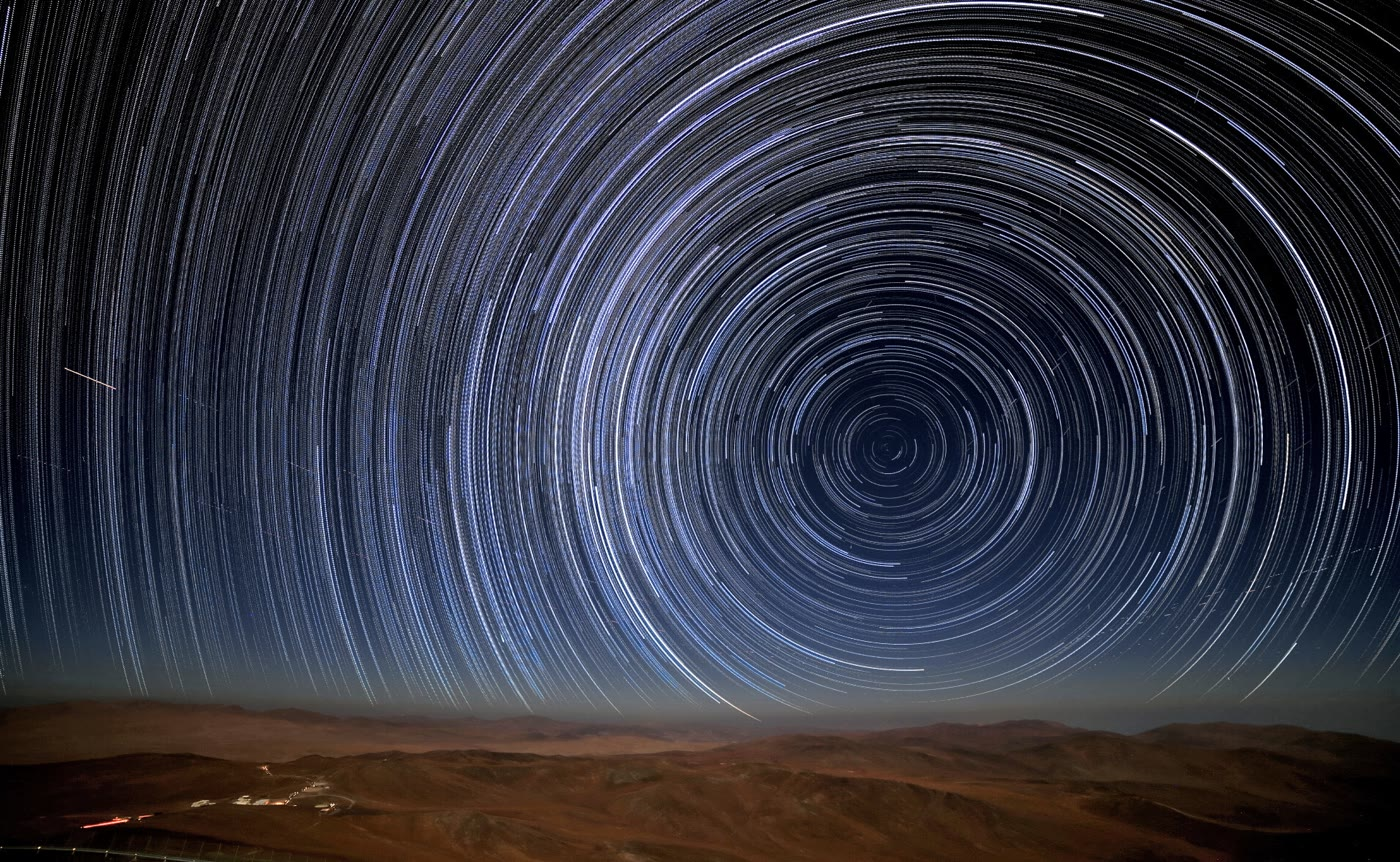
\includegraphics[width=0.8\linewidth]{images/book3/b1-star-trails-paranal.jpg}
% ledger: commons:eso-paranal-star-trails, mpc:paranal

{\small Sterrensporen boven het observatorium van Paranal, in de Atacamawoestijn,
op breedte \ang{24.6} Z: een lange belichting legt de boog van elke ster rond
de zuidelijke \omterm{def:b1:spherical-astronomy:celestial-sphere}{hemelpool} vast, die \ang{24.6} boven de zuidelijke horizon
staat. Foto R.~Wesson/ESO, CC BY 4.0.}
\end{omfigure}

\section{Sterrentijd en zonnetijd}

\begin{definition}[De ecliptica]\label{def:b1:spherical-astronomy:ecliptic}
De \emph{ecliptica}\index{ecliptica} is de \omterm{def:b1:spherical-astronomy:spherical-triangle}{grootcirkel} van de \omterm{def:b1:spherical-astronomy:celestial-sphere}{hemelbol} langs
welke de zon in een jaar schijnbaar beweegt, het spoor van het vlak van de
baan van de aarde. Zij helt over de \omterm{def:b1:spherical-astronomy:celestial-sphere}{hemelevenaar} met de
\emph{schuinte van de ecliptica}\index{schuinte van de ecliptica}
$\varepsilon$, de kanteling van de aardas ten opzichte van haar baan. De
ecliptica snijdt de evenaar in twee punten; het \emph{lentepunt}\index{lentepunt}
$\gamma$ is het punt waar de zon in maart de evenaar noordwaarts kruist. De
ecliptische lengte $\lambda_\odot$ van de zon is
haar hoek langs de ecliptica, vanaf $\gamma$ gemeten, naar het oosten.
\end{definition}

% ledger: earth:obliquity (23.44)
De schuinte is vandaag $\varepsilon = \ang{23.44}$.

\begin{definition}[Sterrentijd]\label{def:b1:spherical-astronomy:sidereal-time}
De plaatselijke \emph{sterrentijd}\index{sterrentijd} is de \omterm{def:b1:spherical-astronomy:equatorial}{uurhoek} van het
\omterm{def:b1:spherical-astronomy:ecliptic}{lentepunt} $\gamma$. Een sterrendag is het tijdsinterval tussen twee passages
van $\gamma$ over de meridiaan.
\end{definition}

Omdat de \omterm{def:b1:spherical-astronomy:equatorial}{rechte klimming} vanaf $\gamma$ oostwaarts wordt geteld en de \omterm{def:b1:spherical-astronomy:equatorial}{uurhoek}
vanaf de meridiaan westwaarts, geldt voor elke ster
\[
  H = \mathrm{LST} - \alpha ,
\]
waarin LST de plaatselijke \omterm{def:b1:spherical-astronomy:sidereal-time}{sterrentijd} is: een ster kruist de meridiaan wanneer
de \omterm{def:b1:spherical-astronomy:sidereal-time}{sterrentijd} gelijk is aan haar \omterm{def:b1:spherical-astronomy:equatorial}{rechte klimming}. Een sterrenklok van een
observatorium laat in één oogopslag zien welk deel van de hemel boven het hoofd
staat.

\begin{proposition}[Sterrendagen en zonnedagen]\label{prop:b1:spherical-astronomy:sidereal-day}
In één \omterm{def:b1:spherical-astronomy:tropical-year}{tropisch jaar} van $N$ gemiddelde zonnedagen draait de aarde $N + 1$ keer
ten opzichte van de sterren. De sterrendag duurt dus
\[
  \frac{N}{N + 1}\times\qty{24}{h},
\]
en met $N = 365.2422$ is dat \qty{23}{h}~\qty{56}{min}~\qty{4.09}{s}: een ster
kruist de meridiaan elke dag \qty{3}{min}~\qty{56}{s} \omterm{def:b1:spherical-astronomy:solar-time}{gemiddelde zonnetijd}
eerder.
\end{proposition}

\begin{proof}
% ledger: usno:tropical-year, earth:Trot (23.9345 h)
Tel de omwentelingen ten opzichte van de zon en ten opzichte van de sterren
over één jaar. De zon beweegt in een jaar één keer oostwaarts langs de
\omterm{def:b1:spherical-astronomy:ecliptic}{ecliptica}, in de richting van de draaiing van de aarde. Ten opzichte van de zon
maakt de aarde dus één omwenteling minder dan ten opzichte van de sterren:
$N$ zonnedagen en $N + 1$ sterrendagen vullen hetzelfde jaar. De sterrendag is
$N/(N+1)$ van een zonnedag, dat wil zeggen
$\qty{86400}{s}\times 365.2422/366.2422 = \qty{86164.09}{s}$; het verschil is
$\qty{235.9}{s}$. Dit stemt overeen met de gemeten draaiingstijd van de aarde ten
opzichte van de sterren, \qty{23.9345}{h}.
\end{proof}

\begin{definition}[Zonnetijd]\label{def:b1:spherical-astronomy:solar-time}
De \emph{ware zonnetijd}\index{ware zonnetijd} is de \omterm{def:b1:spherical-astronomy:equatorial}{uurhoek} van de zon plus
twaalf uur: een zonnewijzer toont die, en het is middag wanneer de zon de
meridiaan kruist. De \emph{gemiddelde zonnetijd}\index{gemiddelde zonnetijd} is
de \omterm{def:b1:spherical-astronomy:equatorial}{uurhoek}, plus twaalf uur, van een fictieve gemiddelde zon die langs de
\omterm{def:b1:spherical-astronomy:celestial-sphere}{hemelevenaar} met een constante snelheid beweegt en in een \omterm{def:b1:spherical-astronomy:tropical-year}{tropisch jaar} één
omwenteling maakt. Hun verschil, ware minus gemiddeld, is de
\emph{tijdsvereffening}\index{tijdsvereffening}.
\end{definition}

De ware zon loopt voor en achter op de gemiddelde zon, om twee redenen. De aarde
beweegt nabij het perihelium, begin januari, sneller dan nabij het aphelium, zodat
de voortgang van de zon langs de \omterm{def:b1:spherical-astronomy:ecliptic}{ecliptica} ongelijkmatig is (de tweede wet van
Kepler). En de zon beweegt langs de \omterm{def:b1:spherical-astronomy:ecliptic}{ecliptica}, die schuin op de evenaar staat,
zodat zelfs een gelijkmatige beweging langs de \omterm{def:b1:spherical-astronomy:ecliptic}{ecliptica} op de evenaar een
ongelijkmatige projectie geeft (de \omterm{def:b1:spherical-astronomy:equatorial}{uurhoek} meet dat) --- sneller nabij de
zonnewendes dan nabij de equinoxen. Burgerlijke klokken houden de \omterm{def:b1:spherical-astronomy:solar-time}{gemiddelde
zonnetijd} op een referentiemeridiaan van hun tijdzone; de plaatselijke
gemiddelde tijd op \omterm{def:b1:spherical-astronomy:geographic}{lengtegraad} $\lambda$ loopt vóór op de tijd in Greenwich met
$\lambda/\ang{15}$ uur.

\begin{omfigure}
\begin{tikzpicture}
\begin{axis}[omrecord, width=0.9\linewidth, height=5.2cm, xmin=0, xmax=365,
  xtick={0,31,59,90,120,151,181,212,243,273,304,334,365},
  xticklabels={J,F,M,A,M,J,J,A,S,O,N,D,},
  ylabel={tijdsvereffening (min)}, ymin=-20, ymax=21,
  tick label style={font=\scriptsize}, label style={font=\small}]
\addplot[black!50, line width=0.4pt] coordinates {(0,0) (365,0)};
\addplot[omDef, line width=1.1pt] table[x=day, y=eot_min] {figdata/out/bachelor-1-day_length-eot.dat};
\node[font=\scriptsize, above, fill=white, inner sep=1pt] at (axis cs:306,16.6) {$+16.4$};
\node[font=\scriptsize, below, fill=white, inner sep=1pt] at (axis cs:41,-14.4) {$-14.2$};
\end{axis}
\end{tikzpicture}

{\small De \omterm{def:b1:spherical-astronomy:solar-time}{tijdsvereffening} over het jaar (ware minus \omterm{def:b1:spherical-astronomy:solar-time}{gemiddelde zonnetijd}): een
zonnewijzer loopt tot \qty{16.4}{min} voor begin november en tot
\qty{14.2}{min} achter half februari. Berekend uit een Kepler-baan met de
excentriciteit 0.0167, de schuinte \ang{23.44}, de lengte van het perihelium en
de datum van de lentenachtevening van 2026.}
% ledger: earth:ecc, earth:obliquity, nasa:earth-perihelion-longitude, usno:seasons-2026
\end{omfigure}

\section{Opkomst, ondergang en de zon}

\begin{proposition}[Opkomst en ondergang]\label{prop:b1:spherical-astronomy:rising}
Op breedte $\varphi$ gaat een ster met \omterm{def:b1:spherical-astronomy:equatorial}{declinatie} $\delta$ die op- en
ondergaat door de horizon bij de \omterm{def:b1:spherical-astronomy:equatorial}{uurhoeken} $\pm H_0$, met
\[
  \cos H_0 = -\tan\varphi\tan\delta ,
\]
bij het \omterm{def:b1:spherical-astronomy:horizontal}{azimut} $\mathrm{A}_0$ met $\cos\mathrm{A}_0 = \sin\delta/\cos\varphi$
(bij opkomst; bij ondergang is het \omterm{def:b1:spherical-astronomy:horizontal}{azimut} $\ang{360} - \mathrm{A}_0$). Zij blijft
boven de horizon gedurende $2H_0$, omgerekend in uren van \ang{15} per uur.
\end{proposition}

\begin{proof}
Op de horizon geldt $h = 0$, en \cref{prop:b1:spherical-astronomy:transform}
geeft $0 = \sin\varphi\sin\delta + \cos\varphi\cos\delta\cos H_0$, en
$\cos\mathrm{A}_0 = \sin\delta/\cos\varphi$. De \omterm{def:b1:spherical-astronomy:equatorial}{uurhoek} neemt gelijkmatig toe,
met \ang{15} per uur, van $-H_0$ bij de opkomst tot $+H_0$ bij de ondergang.
\end{proof}

Voor de zon geeft dit de lengte van de dag, als de zon als een punt wordt
beschouwd en de breking van het licht door de lucht wordt genegeerd (beide
voegen enkele minuten daglicht toe). Op de equinoxen geldt $\delta = 0$,
$H_0 = \ang{90}$: dag en nacht duren overal twaalf uur, en de zon komt recht
in het oosten op.

\begin{omfigure}
\begin{tikzpicture}
\begin{axis}[omrecord, width=0.85\linewidth, height=5.6cm, xmin=40, xmax=320, ymin=0, ymax=75,
  xtick={45,90,135,180,225,270,315}, xticklabels={NE,E,SE,S,SW,W,NW}, ytick={0,15,30,45,60,75},
  xlabel={azimut}, ylabel={hoogte van de zon ($^\circ$)},
  tick label style={font=\scriptsize}, label style={font=\small}]
\addplot[omThm, line width=1pt] table[x=az_deg, y=alt_deg] {figdata/out/bachelor-1-sun_paths-june.dat};
\addplot[black, line width=1pt] table[x=az_deg, y=alt_deg] {figdata/out/bachelor-1-sun_paths-equinox.dat};
\addplot[omDef, line width=1pt] table[x=az_deg, y=alt_deg] {figdata/out/bachelor-1-sun_paths-december.dat};
\begin{scope}[font=\scriptsize, fill=white, fill opacity=0.8, text opacity=1, inner sep=1pt]
  \node[omThm, above, fill=white] at (axis cs:180,68.4) {zomerzonnewende, $\ang{68.4}$};
  \node[above, fill=white] at (axis cs:180,45) {equinoxen, $\ang{45}$};
  \node[omDef, above, fill=white] at (axis cs:180,21.6) {winterzonnewende, $\ang{21.6}$};
\end{scope}
\end{axis}
\end{tikzpicture}

{\small De baan van de zon over de hemel op breedte \ang{45} N op de
zomerzonnewende van juni (rood), de equinoxen (zwart) en de winterzonnewende
van december (blauw), met de middaghoogten $\ang{90} - \varphi + \delta_\odot$.
Op de equinoxen komt de zon recht in het oosten op en gaat zij recht in het
westen onder; in juni komt zij op in het noordoosten.}
\end{omfigure}

\begin{proposition}[De declinatie van de zon]\label{prop:b1:spherical-astronomy:sun-declination}
Wanneer de zon op de ecliptische lengte $\lambda_\odot$ staat, voldoen haar
\omterm{def:b1:spherical-astronomy:equatorial}{declinatie} en \omterm{def:b1:spherical-astronomy:equatorial}{rechte klimming} aan
\[
  \sin\delta_\odot = \sin\varepsilon\sin\lambda_\odot, \qquad
  \tan\alpha_\odot = \cos\varepsilon\tan\lambda_\odot .
\]
\end{proposition}

\begin{proof}
Neem assen met $x$ naar $\gamma$ en $z$ naar de noordelijke \omterm{def:b1:spherical-astronomy:celestial-sphere}{hemelpool}.
In assen $x$, $y'$, $z'$ die aan de \omterm{def:b1:spherical-astronomy:ecliptic}{ecliptica} zijn verbonden, met $z'$ naar haar
pool, is de richting van de zon $(\cos\lambda_\odot, \sin\lambda_\odot, 0)$. De
assen van de \omterm{def:b1:spherical-astronomy:ecliptic}{ecliptica} zijn die van de evenaar, gedraaid over de hoek
$\varepsilon$ om $x$; in de evenaarsassen is de richting van de zon dus
$(\cos\lambda_\odot,\ \sin\lambda_\odot\cos\varepsilon,\
\sin\lambda_\odot\sin\varepsilon)$. Haar $z$-component is $\sin\delta_\odot$;
de verhouding van haar $y$- en $x$-componenten is $\tan\alpha_\odot$.
\end{proof}

\begin{omfigure}
\begin{tikzpicture}
\begin{axis}[omrecord, width=0.9\linewidth, height=6cm, xmin=0, xmax=365, ymin=0, ymax=24,
  xtick={0,31,59,90,120,151,181,212,243,273,304,334,365},
  xticklabels={J,F,M,A,M,J,J,A,S,O,N,D,}, ytick={0,6,12,18,24},
  ylabel={daglengte (h)}, tick label style={font=\scriptsize}, label style={font=\small},
  legend style={font=\scriptsize, at={(0.5,1.02)}, anchor=south, draw=none}, legend columns=5,
  legend cell align=left]
\addplot[black, line width=0.9pt] table[x=day, y=lat0] {figdata/out/bachelor-1-day_length-lengths.dat};
\addplot[omDef, line width=0.9pt] table[x=day, y=lat30] {figdata/out/bachelor-1-day_length-lengths.dat};
\addplot[omThm, line width=0.9pt] table[x=day, y=lat45] {figdata/out/bachelor-1-day_length-lengths.dat};
\addplot[omField, line width=0.9pt] table[x=day, y=lat60] {figdata/out/bachelor-1-day_length-lengths.dat};
\addplot[black, line width=0.9pt, densely dashed] table[x=day, y=lat70] {figdata/out/bachelor-1-day_length-lengths.dat};
\legend{\ang{0}, \ang{30} N, \ang{45} N, \ang{60} N, \ang{70} N}
\end{axis}
\end{tikzpicture}

{\small Lengte van de dag (middelpunt van de zon boven de geometrische horizon)
gedurende het jaar op vijf noordelijke breedten, volgens
\cref{prop:b1:spherical-astronomy:rising,prop:b1:spherical-astronomy:sun-declination}.
Op \ang{70} N blijft de zon weken lang boven de horizon rond de
zomerzonnewende van juni en blijft zij beneden de horizon rond de
winterzonnewende van december. Op het zuidelijk halfrond zijn de krommen met
een half jaar verschoven.}
\end{omfigure}

\begin{definition}[Insolatie]\label{def:b1:spherical-astronomy:insolation}
De \emph{insolatie}\index{insolatie} op een plaats en een tijdstip is het
vermogen van het zonlicht dat per oppervlakte-eenheid van een horizontaal
oppervlak aan de bovenkant van de atmosfeer ontvangen wordt. Met $S_0$ de
zonnestraling op de gemiddelde afstand $a$ van de zon, $r$ de werkelijke afstand
en $\theta_z$ de zenithoek van de zon,
\[
  I = S_0\left(\frac{a}{r}\right)^{2}\cos\theta_z = S_0\left(\frac{a}{r}\right)^{2}\sin h_\odot
  \quad (h_\odot > 0), \qquad I = 0 \text{ 's nachts}.
\]
\end{definition}

% ledger: earth:TSI (1361 W/m2), earth:peri, earth:aph, earth:a
De factor $(a/r)^2$ is de kwadratenwet voor licht (de natuurkundeboeken); de
factor $\cos\theta_z$ komt doordat een bundel met een dwarsdoorsnede van één
vierkante meter zich uitspreidt over $1/\cos\theta_z$ vierkante meter
horizontale grond. Met $S_0 = \qty{1361}{W.m^{-2}}$ en een afstand tussen zon
en aarde van \qty{147.1e6}{km} in het perihelium en \qty{152.1e6}{km} in het
aphelium, varieert de factor $(a/r)^2$ in het jaar met $\pm\qty{3.4}{\percent}$.
De kanteling van de as doet veel meer: zij verandert zowel de middaghoogte als
de lengte van de dag, en die twee samen maken de seizoenen. De dagelijkse en
jaarlijkse sommen van de \omterm{def:b1:spherical-astronomy:insolation}{insolatie}, die het klimaat aandrijven, worden berekend
in \cref{ch:b1:radiation-heat-transport}.


\section{Kalenders}

\begin{definition}[Tropisch jaar]\label{def:b1:spherical-astronomy:tropical-year}
Het \emph{tropisch jaar}\index{tropisch jaar} is het gemiddelde tijdsinterval
tussen twee passages van de zon door het \omterm{def:b1:spherical-astronomy:ecliptic}{lentepunt}. Het bepaalt de seizoenen; het
duurt 365.2422 gemiddelde zonnedagen.
\end{definition}

% ledger: usno:tropical-year, earth:Psid (365.256 d)
Het \omterm{def:b1:spherical-astronomy:tropical-year}{tropisch jaar} is ongeveer twintig minuten korter dan het siderische jaar, de
tijd die de aarde nodig heeft om terug te keren naar dezelfde plaats tussen de
sterren (365.256 dagen), omdat de aardas langzaam draait --- zij presedeert ---
en het \omterm{def:b1:spherical-astronomy:ecliptic}{lentepunt} langs de \omterm{def:b1:spherical-astronomy:ecliptic}{ecliptica} terugvoert (Boek 4). Een kalender moet een geheel aantal dagen passen op het
\omterm{def:b1:spherical-astronomy:tropical-year}{tropisch jaar}, zodat de seizoenen op dezelfde datums terugkomen.

\begin{proposition}[Het Gregoriaanse jaar]\label{prop:b1:spherical-astronomy:gregorian}
In de Gregoriaanse kalender is een jaar een schrikkeljaar van 366 dagen als zijn
getal deelbaar is door 4, behalve de eeuwjaren, die alleen schrikkeljaar zijn
als zij deelbaar zijn door 400. Het gemiddelde jaar is
\[
  365 + \frac14 - \frac1{100} + \frac1{400} = \num{365.2425}\text{ dagen},
\]
en het loopt met de seizoenen één dag achter in ongeveer 3300 jaar.
\end{proposition}

\begin{proof}
% ledger: usno:leap-rule, usno:tropical-year
In 400 jaar zijn er 100 jaren die deelbaar zijn door 4; daarvan zijn er vier
eeuwjaren, waarvan er drie niet deelbaar zijn door 400. Er zijn dus 97
schrikkeljaren en $400\times 365 + 97 = 146\,097$ dagen, dat wil zeggen
365.2425 dagen per jaar. Ten opzichte van een \omterm{def:b1:spherical-astronomy:tropical-year}{tropisch jaar} van 365.2422 dagen
is het overschot 0.0003 dagen per jaar: één dag in $1/0.0003 \approx 3300$ jaar.
\end{proof}

\begin{history}[De kalenderhervorming van 1582]
% ledger: usno:gregorian-1582
De Juliaanse kalender, van Romeinse oorsprong, voegde elk vierde jaar een
schrikkeldag toe: haar jaar van 365.25 dagen is langer dan het \omterm{def:b1:spherical-astronomy:tropical-year}{tropisch jaar} met
0.0078 dagen, één dag in 128 jaar. Na verloop van tijd verschoof de datum van
het \omterm{def:b1:spherical-astronomy:ecliptic}{lentepunt} weg van 21 maart, de datum waarop de berekening van Pasen steunde.
In 1582 voerde paus Gregorius~XIII de kalender in die zijn naam draagt. Deze
kalender schrapte de opgehoopte dagen in één keer en verving de Juliaanse regel
door die van \cref{prop:b1:spherical-astronomy:gregorian}. Zij is intussen de
internationaal aanvaarde burgerlijke kalender.
\end{history}

\begin{inthefield}[Een positie bepalen met de sterren]
Vóór de satellietnavigatie bepaalden zeevaarders hun breedte- en \omterm{def:b1:spherical-astronomy:geographic}{lengtegraad}
met de hemel. Met een sextant mat men de \omterm{def:b1:spherical-astronomy:horizontal}{hoogte} van de zon om het middaguur, of
van twee of drie sterren bij de schemering, en las men de tijd af op een
chronometer die de tijd van de Greenwichmeridiaan bijhield. Elke \omterm{def:b1:spherical-astronomy:horizontal}{hoogte} geeft,
samen met de \omterm{def:b1:spherical-astronomy:equatorial}{declinatie} van de ster en haar \omterm{def:b1:spherical-astronomy:equatorial}{uurhoek} te Greenwich uit een
almanak, een \omterm{def:b1:spherical-astronomy:spherical-triangle}{kleine cirkel} op de aarde waarop het schip ligt: de verzameling
punten waar de ster op die \omterm{def:b1:spherical-astronomy:horizontal}{hoogte} staat. Twee of drie van zulke cirkels snijden
elkaar in de positie van het schip --- bolvormige trigonometrie die elke dag op
zee werd opgelost. De middaghoogte van de zon alleen geeft de \omterm{def:b1:spherical-astronomy:geographic}{breedtegraad}
(\cref{prop:b1:spherical-astronomy:culmination}); de kloktijd van het plaatselijke
middaguur geeft de \omterm{def:b1:spherical-astronomy:geographic}{lengtegraad}, tegen vier minuten tijd per graad.
\begin{center}
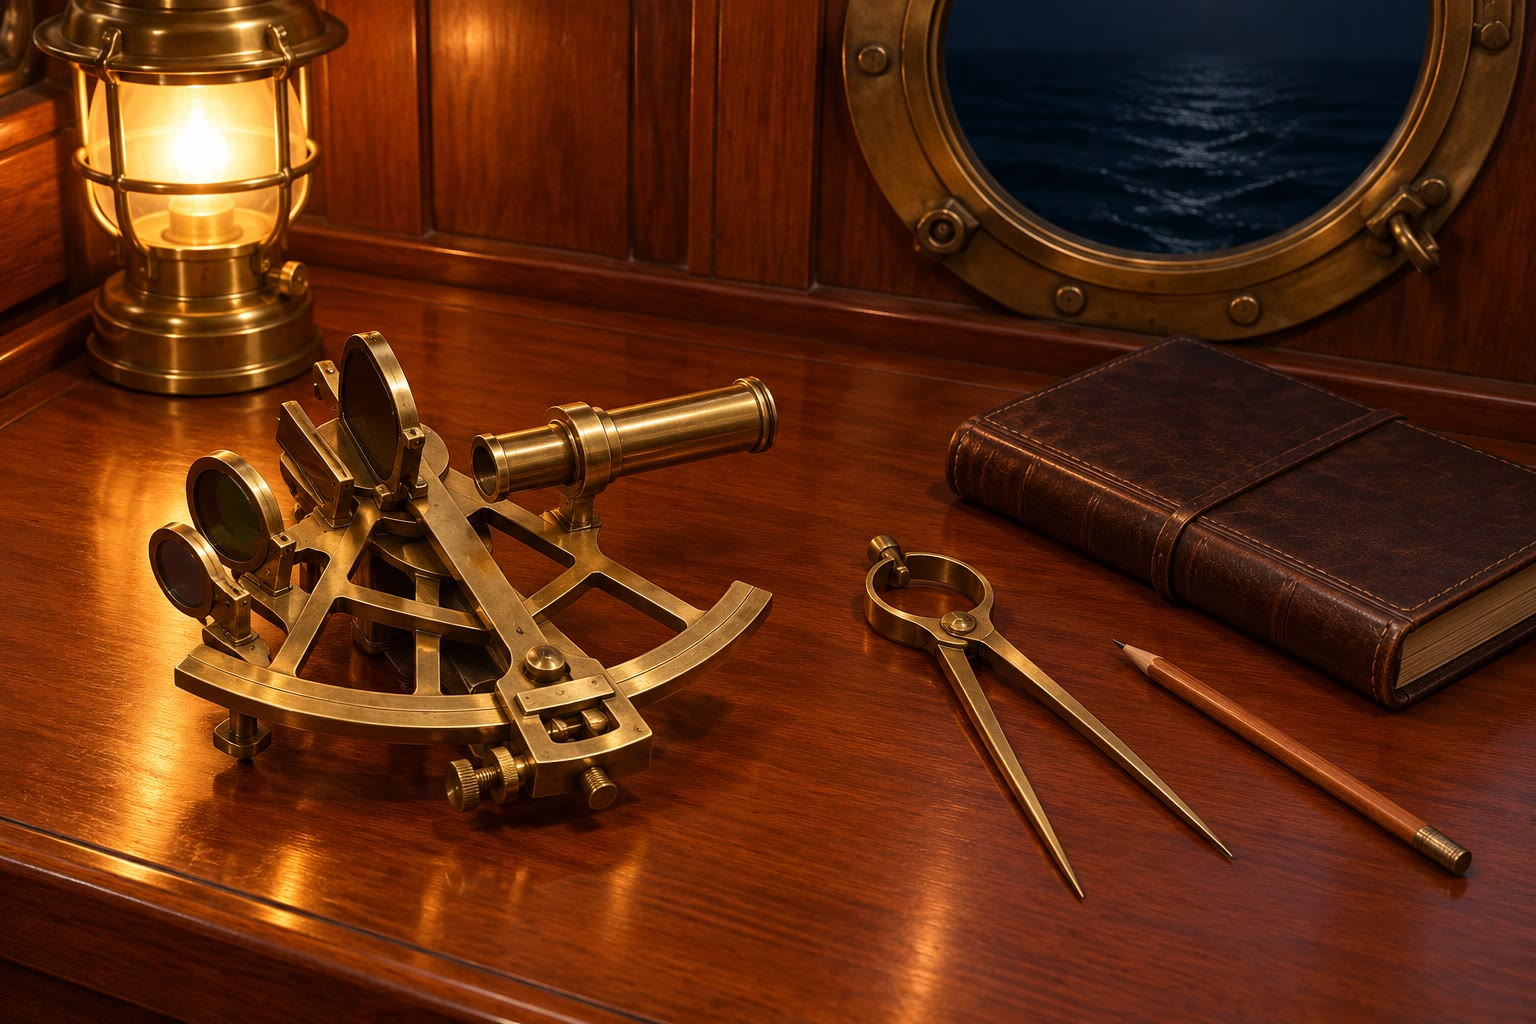
\includegraphics[width=0.55\linewidth]{images/book3/ai/b1-sextant.jpg}
\end{center}
\end{inthefield}

\section{Oefeningen}

\begin{exercise}[$\star$]\label{exo:b1:spherical-astronomy:1}
Een waarnemer bevindt zich op breedte \ang{52} N. Op welke \omterm{def:b1:spherical-astronomy:horizontal}{hoogte} staat de
noordelijke \omterm{def:b1:spherical-astronomy:celestial-sphere}{hemelpool}? Welke sterren gaan er door hun \omterm{def:b1:spherical-astronomy:equatorial}{declinatie} nooit onder,
en welke komen er nooit op?
\end{exercise}

\begin{exercise}[$\star$]\label{exo:b1:spherical-astronomy:2}
Reken een \omterm{def:b1:spherical-astronomy:equatorial}{rechte klimming} van \qty{6}{h}~\qty{45}{min} om in graden. Wat is bij
een plaatselijke \omterm{def:b1:spherical-astronomy:sidereal-time}{sterrentijd} van \qty{10}{h}~\qty{0}{min} de \omterm{def:b1:spherical-astronomy:equatorial}{uurhoek} van een
ster met die \omterm{def:b1:spherical-astronomy:equatorial}{rechte klimming}? Staat de ster oost of west van de meridiaan?
\end{exercise}

\begin{exercise}[$\star$]\label{exo:b1:spherical-astronomy:3}
Bereken op breedte \ang{40} N de middaghoogte van de zon op de twee
zonnewendes en op de equinoxen ($\varepsilon = \ang{23.44}$).
\end{exercise}

\begin{exercise}[$\star$]\label{exo:b1:spherical-astronomy:4}
Was 1900 een schrikkeljaar? Was 2000 dat? Wordt 2100 dat? Met hoeveel dagen
per eeuw loopt de Juliaanse kalender achter op een \omterm{def:b1:spherical-astronomy:tropical-year}{tropisch jaar} van 365.2422
dagen, en met hoeveel de Gregoriaanse?
\end{exercise}

\begin{exercise}[$\star\star$]\label{exo:b1:spherical-astronomy:5}
Twee punten liggen op breedte \ang{45} N, op lengtegraden \ang{0} en
\ang{90} O. Bereken de afstand over de \omterm{def:b1:spherical-astronomy:spherical-triangle}{grootcirkel} tussen hen
($R = \qty{6371}{km}$) en de afstand langs hun parallel. Welke is korter, en met
hoeveel?
\end{exercise}

\begin{exercise}[$\star\star$]\label{exo:b1:spherical-astronomy:6}
Op breedte \ang{48} N heeft een ster met \omterm{def:b1:spherical-astronomy:equatorial}{declinatie} \ang{20} de \omterm{def:b1:spherical-astronomy:equatorial}{uurhoek}
\ang{30}. Bereken haar \omterm{def:b1:spherical-astronomy:horizontal}{hoogte} en haar \omterm{def:b1:spherical-astronomy:horizontal}{azimut}. In welke richting moet de
waarnemer kijken?
\end{exercise}

\begin{exercise}[$\star\star$]\label{exo:b1:spherical-astronomy:7}
Bereken de lengte van de dag op breedte \ang{60} N op de zomerzonnewende van
juni, waarbij de zon als een punt op een geometrische horizon wordt beschouwd.
Controleer het antwoord met de figuur van de dagslengte.
\end{exercise}

\begin{exercise}[$\star\star$]\label{exo:b1:spherical-astronomy:8}
Een ster kruist vanavond om 22:00 uur plaatselijke gemiddelde tijd de
meridiaan. Wanneer kruist zij de meridiaan over dertig dagen? Na hoeveel dagen
kruist zij de meridiaan op het middaguur, onzichtbaar in het daglicht?
\end{exercise}

\begin{exercise}[$\star\star$]\label{exo:b1:spherical-astronomy:9}
Bereken de \omterm{def:b1:spherical-astronomy:insolation}{insolatie} aan de bovenkant van de atmosfeer om het middaguur op
breedte \ang{45} N (a) op een equinox, met $r = a$; (b) op de zomerzonnewende
van juni, met voor $r$ de afstand in het aphelium. Gegevens: $S_0 = \qty{1361}{W.m^{-2}}$,
$a = \qty{149.598e6}{km}$, aphelium \qty{152.100e6}{km}.
\end{exercise}

\begin{exercise}[$\star\star\star$]\label{exo:b1:spherical-astronomy:10}
Bereken met \cref{prop:b1:spherical-astronomy:sun-declination} de \omterm{def:b1:spherical-astronomy:equatorial}{declinatie} en
de \omterm{def:b1:spherical-astronomy:equatorial}{rechte klimming} van de zon wanneer haar ecliptische lengte \ang{60} is. Met
hoeveel graden blijft de \omterm{def:b1:spherical-astronomy:equatorial}{rechte klimming} achter op de lengte? Leg met dit
resultaat uit waarom de helling van de \omterm{def:b1:spherical-astronomy:ecliptic}{ecliptica} bijdraagt aan de
\omterm{def:b1:spherical-astronomy:solar-time}{tijdsvereffening}.
\end{exercise}

\begin{exercise}[$\star\star\star$]\label{exo:b1:spherical-astronomy:11}
Toon aan dat op de zomerzonnewende de zon opkomt op het \omterm{def:b1:spherical-astronomy:horizontal}{azimut} $\mathrm{A}_0$
met $\cos\mathrm{A}_0 = \sin\varepsilon/\cos\varphi$. Op welke breedte komt zij
precies in het noordoosten op? Wat gebeurt er met de formule op breedten boven
$\ang{90} - \varepsilon$?
\end{exercise}

\begin{exercise}[$\star\star\star$]\label{exo:b1:spherical-astronomy:12}
Een bolvormige tweehoek is het deel van een bol tussen twee halve \omterm{def:b1:spherical-astronomy:spherical-triangle}{grootcirkels}
die twee tegenoverliggende punten verbinden, onder de hoek $\theta$ ten opzichte
van elkaar. (a) Toon aan dat haar oppervlakte $2\theta R^2$ is. (b) Elke zijde
van een \omterm{def:b1:spherical-astronomy:spherical-triangle}{sferische driehoek} $ABC$, tot een volledige \omterm{def:b1:spherical-astronomy:spherical-triangle}{grootcirkel} doorgetrokken,
geeft met de andere twee drie paren van tegenoverliggende tweehoeken met hoeken
$A$, $B$, $C$ die de bol bedekken; de driehoek en haar tegenoverliggende worden
drie keer bedekt. Leid hieruit de stelling van Girard af: de oppervlakte van de
driehoek is $R^2(A + B + C - \pi)$. (c) Pas die toe op de driehoek met drie
rechte hoeken en op de driehoek uit dit hoofdstuk (hoeken \ang{89.9},
\ang{64.9}, \ang{67.4}).
\end{exercise}

\section{Probleem: Een nacht op een bergobservatorium}

\begin{problem}[{Weekendprobleem --- waar het Paranal-observatorium staat, wat de hemel er toont en hoe lang de langste nacht duurt}]
\label{pb:b1:spherical-astronomy:1}
% ledger: mpc:paranal, mpc:greenwich, simbad:sirius, simbad:canopus, usno:seasons-2026, earth:obliquity, usno:tropical-year
% numbers computed in the scratch calculator calc/ch01.py from the rounded data
Het Paranal-observatorium staat in de Atacamawoestijn op breedte \ang{24.63} Z,
\omterm{def:b1:spherical-astronomy:geographic}{lengtegraad} \ang{70.40} W. Het Royal Observatory te Greenwich, waarvandaan de
lengtegraden worden geteld, ligt op \ang{51.48} N, \ang{0.00}. Twee heldere
sterren van de zuidelijke hemel hebben de coördinaten
\begin{center}
\small
\begin{tabular}{lcc}
\hline
ster & \omterm{def:b1:spherical-astronomy:equatorial}{rechte klimming} & \omterm{def:b1:spherical-astronomy:equatorial}{declinatie} \\
\hline
Sirius & \qty{6}{h}~\qty{45}{min}~\qty{9}{s} & \ang{-16.72} \\
Canopus & \qty{6}{h}~\qty{23}{min}~\qty{57}{s} & \ang{-52.70} \\
\hline
\end{tabular}
\end{center}
Neem $R = \qty{6371}{km}$, $\varepsilon = \ang{23.44}$, een \omterm{def:b1:spherical-astronomy:tropical-year}{tropisch jaar} van
365.2422 dagen, en beschouw de zon als een punt op een geometrische horizon.

\medskip
\noindent\textbf{Deel I --- Paranal op de bol.}
\begin{enumerate}
  \item Geef de poolafstanden van Paranal en Greenwich, en hun verschil in
        \omterm{def:b1:spherical-astronomy:geographic}{lengtegraad}.
  \item Schrijf de cosinusregel op voor de driehoek noordpool--Paranal--Greenwich
        en bereken de cosinus van de hoekafstand $\Delta$ tussen de twee
        observatoria.
  \item Leid hieruit $\Delta$ in graden af en de afstand over de \omterm{def:b1:spherical-astronomy:spherical-triangle}{grootcirkel} in
        kilometers.
  \item Bereken de beginkoers vanaf Paranal naar Greenwich
        (\cref{met:b1:spherical-astronomy:great-circle}).
  \item Controleer de koers met de sinusregel.
  \item Zou een vliegtuig dat deze koers de hele weg aanhoudt Greenwich bereiken?
        Leg uit.
\end{enumerate}

\medskip
\noindent\textbf{Deel II --- De hemel van Paranal.}
\begin{enumerate}[resume]
  \item Op welke \omterm{def:b1:spherical-astronomy:horizontal}{hoogte} staat de zuidelijke \omterm{def:b1:spherical-astronomy:celestial-sphere}{hemelpool} boven de zuidelijke
        horizon van Paranal?
  \item Op welke \omterm{def:b1:spherical-astronomy:horizontal}{hoogte} kruist Sirius de meridiaan, en aan welke kant van het
        \omterm{def:b1:spherical-astronomy:celestial-sphere}{zenit}?
  \item Beneden welke \omterm{def:b1:spherical-astronomy:equatorial}{declinatie} is een ster op Paranal circumpolair? Is Canopus
        circumpolair?
  \item Welke hoogste \omterm{def:b1:spherical-astronomy:horizontal}{hoogte} bereikt Canopus?
  \item Bereken de \omterm{def:b1:spherical-astronomy:equatorial}{uurhoek} waarbij Sirius opkomt, en hoe lang zij boven de
        horizon blijft, in sterrenuren.
  \item Op welk \omterm{def:b1:spherical-astronomy:horizontal}{azimut} komt Sirius op?
\end{enumerate}

\medskip
\noindent\textbf{Deel III --- Klokken.}
\begin{enumerate}[resume]
  \item Wat is de plaatselijke \omterm{def:b1:spherical-astronomy:sidereal-time}{sterrentijd} wanneer Sirius de meridiaan kruist?
  \item Bereken de lengte van de sterrendag, en met hoeveel minuten de
        meridiaanpassage van een ster elke nacht vroeger komt.
  \item Neem de plaatselijke \omterm{def:b1:spherical-astronomy:sidereal-time}{sterrentijd} om middernacht van de plaatselijke
        gemiddelde tijd op \qty{12}{h} bij de lentenachtevening van maart
        (20 maart 2026), wanneer de zon nabij het \omterm{def:b1:spherical-astronomy:ecliptic}{lentepunt} staat; zij neemt
        dan dagelijks $24/365.2422$ uur toe. Hoeveel dagen na de equinox kruist
        Sirius de meridiaan om middernacht van de plaatselijke gemiddelde tijd?
        Op welke datum?
  \item Hoeveel verschilt de plaatselijke gemiddelde tijd van Paranal in die
        nacht van de tijd in Greenwich?
  \item De \omterm{def:b1:spherical-astronomy:solar-time}{tijdsvereffening} is dan ongeveer \qty{-3}{min}. Welke tijd toont een
        zonnewijzer op het observatorium (\omterm{def:b1:spherical-astronomy:solar-time}{ware zonnetijd}) wanneer Sirius de
        meridiaan kruist?
  \item Hoeveel eerder kruist zij de meridiaan een week later?
\end{enumerate}

\medskip
\noindent\textbf{Deel IV --- De langste nacht.}
\begin{enumerate}[resume]
  \item Wat is de \omterm{def:b1:spherical-astronomy:equatorial}{declinatie} van de zon bij elke zonnewende?
  \item Bereken de middaghoogte van de zon op Paranal bij de zonnewendes van juni
        en december. Aan welke kant van het \omterm{def:b1:spherical-astronomy:celestial-sphere}{zenit} staat zij in december?
  \item Bij de winterzonnewende van december is de afstand tussen zon en aarde
        0.9837 keer de gemiddelde afstand. Bereken de \omterm{def:b1:spherical-astronomy:insolation}{insolatie} om het middaguur
        aan de bovenkant van de atmosfeer boven Paranal
        ($S_0 = \qty{1361}{W.m^{-2}}$).
  \item Bij welke zonnewende is de nacht op Paranal het langst? Bereken de
        \omterm{def:b1:spherical-astronomy:equatorial}{uurhoek} van de zonsondergang op die datum.
  \item Op welk \omterm{def:b1:spherical-astronomy:horizontal}{azimut} komt de zon op die datum op?
  \item Leid hieruit de lengte af van de langste nacht van het jaar op Paranal, in
        uren en minuten.
\end{enumerate}
\end{problem}
